% Institute of Computer Science thesis template
% authors: Sven Laur, Liina Kamm, Tõnu Tamme
% last change Eero Vainikko <eero.vainikko@ut.ee> 12.01.2021
%--
% Compilation instructions:
% 1. Choose main language on line 55-56 (English or Estonian)
% 2. Compile 1-3 times to get refences right
% pdflatex unitartucs-thesis-template
% bibtex unitartucs-thesis-template
%--
% Please use references like this:
% <text> <non-breaking-space> <cite/ref-command> <punctuation>
% This is an example~\cite{example}.

\documentclass[12pt]{article}

% A package for setting layout and margins for your thesis 
\usepackage[a4paper]{geometry}

%%=== A4 page setup ===
%\setlength{\paperwidth}{21.0cm} 
%\setlength{\paperheight}{29.7cm}
%\setlength{\textwidth}{16cm}
%\setlength{\textheight}{25cm}


% When you write in Estonian then you want to use text with right character set
% By default LaTeX does not know what to do with õäöu letters. You have to specify
% a correct input and font encoding. For that you have to Google the Web     
%
% For TexShop under MacOS X. The right lines are 
%\usepackage[applemac]{inputenc}
%\usepackage[T1]{fontenc} %Absolutely critical for *hyphenation* of words with non-ASCII letters.
%
% For Windows and Linux the right magic lines are   
% \usepackage[latin1]{inputenc}
% \usepackage[latin5]{inputenc}
%
\usepackage[utf8]{inputenc} %standard encoding since 2018 (can be commented out?)
\usepackage[T1]{fontenc} %Absolutely critical for *hyphenation* of words with non-ASCII letters.

% Typeset text in Times Roman instead of Computer Modern (EC)
\usepackage{times}

% Suggested packages:
\usepackage{microtype}  %towards typographic perfection...
\usepackage{inconsolata} %nicer font for code listings. (Use \ttfamily for lstinline bastype)


% Use package babel for English or Estonian 
% If you use Estonian make sure that Estonian hyphenation is installed 
% - hypen-estonian or eehyp packages
%
%===Choose the main language in thesis
\usepackage[estonian, english]{babel} %the thesis is in English 
%\usepackage[english, estonian]{babel} %the thesis is in Estonian

% Change Babel document elements 
\addto\captionsestonian{%
  \renewcommand{\refname}{Viidatud kirjandus}%
  \renewcommand{\appendixname}{Lisad}%
}

% If you have problems with Estonian keywords in the bibliography
%\usepackage{biblatex}
%\usepackage[backend=biber]{biblatex}
%\usepackage[style=alphabetic]{biblatex}
%% plain --> \usepackage[style=numeric]{biblatex}
%% abbrv --> \usepackage[style=numeric,firstinits=true]{biblatex}
%% unsrt --> \usepackage[style=numeric,sorting=none]{biblatex}
%% alpha --> \usepackage[style=alphabetic]{biblatex}
%\DefineBibliographyStrings{estonian}{and={ja}}
%\addbibresource{unitartucs-thesis.bib}


% General packages for math in general, theorems and symbols 
% Read ftp://ftp.ams.org/ams/doc/amsmath/short-math-guide.pdf for further information
\usepackage{amsmath} 
\usepackage{amsthm}
\usepackage{amssymb}
\usepackage{multirow}
\usepackage{booktabs}
% Optional calligraphic fonts    
% \usepackage[mathscr]{eucal}

% Print a dot instead of colon in table or figure captions
\usepackage[labelsep=period]{caption}

% Packages for building tables and tabulars 
\usepackage{array}
\usepackage{tabu}   % Wide lines in tables
\usepackage{xspace} % Non-eatable spaces in macros
\usepackage{subcaption}
% Including graphical images and setting the figure directory
\usepackage{graphicx}
\graphicspath{{figures/}}

% Packages for getting clickable links in PDF file
%\usepackage{hyperref}
\usepackage[hidelinks]{hyperref} %hide red (blue,green) boxes around links
\usepackage[all]{hypcap}


% Packages for defining colourful text together with some colours
\usepackage{color}
\usepackage{xcolor} 
%\definecolor{dkgreen}{rgb}{0,0.6,0}
%\definecolor{gray}{rgb}{0.5,0.5,0.5}
\definecolor{mauve}{rgb}{0.58,0,0.82}


% Standard package for drawing algorithms
% Since the thesis in article format we must define \chapter for
% the package algorithm2e (otherwise obscure errors occur) 
\let\chapter\section
\usepackage[ruled, vlined, linesnumbered]{algorithm2e}

% Fix a  set of keywords which you use inside algorithms
\SetKw{True}{true}
\SetKw{False}{false}
\SetKwData{typeInt}{Int}
\SetKwData{typeRat}{Rat}
\SetKwData{Defined}{Defined}
\SetKwFunction{parseStatement}{parseStatement}


% Nice todo notes
\usepackage{todonotes}

% comments and verbatim text (code)
\usepackage{verbatim}


% Proper way to create coloured code listings
\usepackage{listings}
\lstset{ 
  %language=python,                % the language of the code
  language=C++,
  basicstyle=\footnotesize,        % the size of the fonts that are used for the code
  %numbers=left,                   % where to put the line-numbers
  %numberstyle=\footnotesize,      % the size of the fonts that are used for the line-numbers
  numberstyle=\tiny\color{gray}, 
  stepnumber=1,                    % the step between two line-numbers. If it's 1, each line 
                                   % will be numbered
  numbersep=5pt,                   % how far the line-numbers are from the code
  backgroundcolor=\color{white},   % choose the background color. You must add \usepackage{color}
  showspaces=false,                % show spaces adding particular underscores
  showstringspaces=false,          % underline spaces within strings
  showtabs=false,                  % show tabs within strings adding particular underscores
  frame = lines,
  %frame=single,                   % adds a frame around the code
  rulecolor=\color{black},		   % if not set, the frame-color may be changed on line-breaks within 
                                   % not-black text (e.g. commens (green here))
  tabsize=2,                       % sets default tabsize to 2 spaces
  captionpos=b,                    % sets the caption-position to bottom
  breaklines=true,                 % sets automatic line breaking
  breakatwhitespace=false,         % sets if automatic breaks should only happen at whitespace
  %title=\lstname,                 % show the filename of files included with \lstinputlisting;
                                   % also try caption instead of title
  keywordstyle=\color{blue},       % keywCurriculumord style
  commentstyle=\color{dkgreen},    % comment style
  stringstyle=\color{mauve},       % string literal style
  escapeinside={\%*}{*)},          % if you want to add a comment within your code
  morekeywords={*,game, fun}       % if you want to add more keywords to the set
}


% Obscure packages to write logic formulae and program semantics
% Unless you do a thesis on program semantics or static code analysis you do not need that
% http://logicmatters.net/resources/ndexamples/proofsty3.html <= writing type rules => use semantic::inference
% ftp://tug.ctan.org/tex-archive/macros/latex/contrib/semantic/semantic.pdf
\usepackage{proof}
\usepackage{semantic} 
\setlength{\inferLineSkip}{4pt}
\def\predicatebegin #1\predicateend{$\Gamma \vdash #1$}

% If you really want to draw figures in LaTeX use packages tikz or pstricks
% However, getting a corresponding illustrations is really painful  


% Define your favorite macros that you use inside the thesis 
% Name followed by non-removable space
\newcommand{\proveit}{ProveIt\xspace}

% Macros that make sure that the math mode is set
\newcommand{\typeF}[1] {\ensuremath{\mathsf{type_{#1}}}\xspace}
\newcommand{\opDiv}{\ensuremath{\backslash \mathsf{div}}\xspace} 

% Nice Todo box
\setlength{\marginparwidth}{2cm}
\newcommand{\TODO}{\todo[inline]}

% A way to define theorems and lemmata
\newtheorem{theorem}{Theorem}



%%% BEGIN DOCUMENT
\begin{document}

%===BEGIN TITLE PAGE
\thispagestyle{empty}
\begin{center}

\large
\iflanguage{english}{%
UNIVERSITY OF TARTU\\
Faculty of Science and Technology\\
Institute of Computer Science\\
Computer Science Curriculum\\
%Software Engineering Curriculum\\
}{%\iflanguage
TARTU ÜLIKOOL\\
Loodus- ja täppisteaduste valdkond\\
Arvutiteaduse instituut\\
Informaatika õppekava\\
}%\iflanguage

%\vspace*{\stretch{5}}
\vspace{25mm}

\Large Chan Wai Tik

\vspace{4mm}

\huge Emergent Theory of Mind (ToM) from Token Merging


%\vspace*{\stretch{7}}
\vspace{20mm}

\Large
\iflanguage{english}{%
%Bachelor's Thesis (9 ECTS)
Master's Thesis (30 ECTS)
}{%\iflanguage
Bakalaureusetöö (9 EAP)
}%\iflanguage

\end{center}

\vspace{2mm}

\begin{flushright}
 {
 \setlength{\extrarowheight}{5pt}
 \begin{tabular}{r l} 
  \sffamily \iflanguage{english}{Supervisor(s)}{Juhendaja(d)}: &                    \sffamily Kallol Roy, Assistant Professor
 \end{tabular}
 }
\end{flushright}

%\vspace*{\stretch{3}}\iflanguage
%\vspace{10mm}

\vfill
\centerline{\large Tartu \the\year}

%===END TITLE PAGE

% If the thesis is printed on both sides of the page then 
% the second page must be must be empty. Comment this out
% if you print only to one side of the page comment this out
%\newpage
%\thispagestyle{empty}    
%\phantom{Text to fill the page}
% END OF EXTRA PAGE WITHOUT NUMBER


%===COMPULSORY INFO PAGE
\newpage

%=== Info in English
\newcommand\EngInfo{{%
\selectlanguage{english}
\noindent\textbf{\large Emergent Theory of Mind (ToM) from Token Merging}

\vspace*{3ex}

\noindent\textbf{Abstract:}

\noindent
To be done

\vspace*{1ex}

\noindent\textbf{Keywords:}\\
\TODO{List of keywords}
%Layout, formatting, template

\vspace*{1ex}

\noindent\textbf{CERCS:}\TODO{CERCS code and name:~\url{https://www.etis.ee/Portal/Classifiers/Details/d3717f7b-bec8-4cd9-8ea4-c89cd56ca46e}}

\vspace*{1ex}
}}%\newcommand\EngInfo


%=== Info in Estonian
\newcommand\EstInfo{{%
\selectlanguage{estonian}
\noindent\textbf{\large Tüübituletus neljandat järku loogikavalemitele}
\vspace*{1ex}

\noindent\textbf{Lühikokkuvõte:} 

%\noindent ...

\TODO{One or two sentences providing a basic introduction to the field, comprehensible to a scientist in
any discipline.}
\TODO{Two to three sentences of
more detailed background, comprehensible to scientists in related disciplines.}
\TODO{One sentence clearly stating the general problem being addressed by this particular
study.}
\TODO{One sentence summarising the main result (with the words ``here we show´´ or their equivalent).}
\TODO{Two or three sentences explaining what
the main result reveals in direct
comparison to what was thought to be the case previously, or how the main result adds to previous knowledge.}
\TODO{One or two sentences to put the results into a more general context.}
\TODO{Two or three sentences to provide a
broader perspective, readily
comprehensible to a scientist in any
discipline, may be included in the first paragraph
if the editor considers that the accessibility of
the paper is significantly enhanced by their inclusion.}

\vspace*{1ex}

\noindent\textbf{Võtmesõnad:}\\
\TODO{List of keywords}
%Layout, formatting, template

\vspace*{1ex}

\noindent\textbf{CERCS:}\TODO{CERCS kood ja nimetus:~\url{https://www.etis.ee/Portal/Classifiers/Details/d3717f7b-bec8-4cd9-8ea4-c89cd56ca46e}}

\vspace*{1ex}
}}%\newcommand\EstInfo


%=== Determine the order of languages on Info page
\iflanguage{english}{\EngInfo}{\EstInfo}
\iflanguage{estonian}{\EngInfo}{\EstInfo}


\newpage
\tableofcontents

% END OF TODO PAGE 


\newpage
\section{Introduction}

The recent development in Large Language Models (LLM) such as ChatCPT has archived huge success and stormed the world  with its capability of solving varieties of tasks solely based on mastery in language training\cite{Bubeck_2023}. However, the underlining mechanism is still unknown and hard to investigate due to the large parameter space. On the other hand, some research\cite{Kosinski_2023} suggested that LLM has developed a sense of the Theory of Mind (ToM) along the way during its language training as a by-product. Those researches drive the research focus of this thesis on how a language model consolidates information from words to become understanding and the generative ability to interact with the outside world.

In linguistics study, the hypothesis proposed by Chomsky\cite{Hauser_2002} suggested there are two senses of faculty of language: internal(I) and external(E) language(details in \ref{introLanguage}), and the study object for linguistics should primarily focus on I-language(though, mind) by modeling from E-language, and this results in the generative grammar. In a high-level overview, the I-language described by Chomsky can be translated into the Theory of Ming(ToM) from psychology, but it is more well defined from the psychology aspect(details in \ref{ToM}) and a large amount of research shows there is a strong correlation between ToM and external language training. However, this type of influence is not captured by the linguistics field.

With all those components described above, this thesis proposes a hypothesis that the learning dynamic for those LLM can be described by the following diagram(\ref{fig:LLMhypothesis}) in a top-level view.
\begin{figure} [!h]
\begin{center}
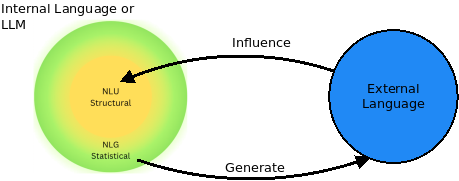
\includegraphics[width=0.8\textwidth]{figures/Ilang_Elang_NLU_NLG.png}
\caption{Hypothesis on LLM's learning dynamic} 
\label{fig:LLMhypothesis}
\end{center}
\end{figure}

The above diagram treats the LLM as the internal language that is composite with two main components from natural language processing(NLP), natural language understanding(NLU), and generation(NLG), with the structure that NLU is supporting NLG and NLG is indirectly influencing back to NLU by external language. 

Since the hypothesis is large in scale, it should be modularized into several parts of research which consist of:
\begin{enumerate}
    \item External Influence on Understanding
    \item Bridging between understanding and generation
    \item Generative and influence back to Understanding
\end{enumerate}
In the thesis, it is focused on the first part of the study.

The paper is organized into 5 sections, the first section is an introduction which will give some overview of the background, followed by two sections of literature review. The experiment details will be described in section four and followed by the result discussion and conclusion.

\subsection{Language} \label{introLanguage}
Language has variate meanings according to different content and setting, as pointed out in\cite{Hauser_2002}, DNA is a universal language that encodes biological information that is shared along all living organisms on earth, but not the case for communication. In the context of communication, human language also got significantly different from other species in its power of expression which is deeply correlated with the property of human language on hierarchy structured(grammar), generative, and most importantly recursive\cite{Hauser_2002}.  The study of language(Linguistics) is integrated with a wide range of scientific areas from mathematics, philosophy, neuroscience, etc\cite{Gallego_2022}. In viewing language from a biological point of view, bio-linguistics treats it as an evolving organism and reshape the study as the internal and external language (I-Language and E-Language)\cite{Gallego_2022}.  I-language is defined to be a mental mind which is intentional, internal, and individual and represents the computational aspect of language while the E-language is the observable language that humans use in communication\cite{Gallego_2022, Hauser_2002}.  
In this formulation, the study of linguistics focuses on inferring the mechanism of  I-language by observing external language generated by internal language and formulating the grammar in daily use. 
The relationship between grammar, I-language, and E-language can be visualized below (fig:\ref{fig:ilanguage}) \cite{Mark_2006}:
\begin{figure} [!h]
\begin{center}
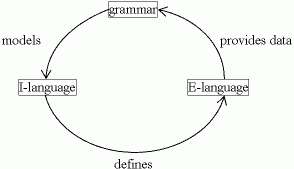
\includegraphics[width=0.4\textwidth]{figures/iLanguage_eLanguage.png}
\caption{relationship between Grammar, I-language and E-language.}
\label{fig:ilanguage}
\end{center}
\end{figure}

One observation of the external language is its property on an infinite set of expressions together with the constraint on limited memory of the brain which suggested that I-language holds an abstract and generative structure behind the scenes and plays a crucial role in determining the interpretation\cite{Tanaka_2019}. From those observations on external language, Chomsky has proposed universal grammar (UG) and minimalist program(MP) to describe and characterize the formulation and property of I-language.\\
UG hypothesized that human language shares a certain degree of fundamental similarities such as general constraints on grammar and common property on features like lexical categories\cite{D_browska_2015}, etc., and this unique grammar follows the three-factor of language design\cite{Chomsky_2005}:
\begin{itemize}
    \item language-independent principles of data processing
    \item structural architecture
    \item computational efficiency
\end{itemize}
Those principles above assert the base of MP. In the framework of MP, it proposes a bare phrase structure(BPS) together with a simple operator - MERGE to construct it.
The MERGE operator is very simple and takes 2 syntactic arguments and combines them to form a new syntactic object:\\
\begin{center} MERGE($\alpha$,$\beta$)= {$K$, {$\alpha$,$\beta$} } \end{center} \\
Here $\alpha$ and $\beta$ are the two arguments and $K$ is the new object often called "label". The most difficult part here is how to determine the label of the new object, detail can be found in \footnote{LIN331 – Syntactic Theory- https://nlacara.github.io/teaching/331S18/331-7-bps.pdf}
Here is a visualization example of BPS and MERGE operation with lexical categories (fig:\ref{fig:bps}):
\begin{figure} [!h]
\begin{center}
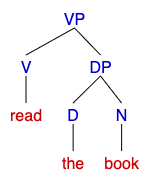
\includegraphics[width=0.2\textwidth]{figures/BSP_merge_lexical.png}
\caption{Example on BPS and MERGE (source\: wiki https\:\/\/en.wikipedia.org\/wiki\/Merge_\%28linguistics\%29} 
\label{fig:bps}
\end{center}
\end{figure}
However, this type of structure can generate syntactically correct but semantically meaningless language as shown by Chomsky in his book " Syntactic Structures".

\newpage
\subsection{Theory of Mind (ToM)}\label{ToM}
Theory of Mind has a long history and is an active research field along a broad range of science like developmental or social  psychology, etc, and neuroscience. In the simplest explanation, it can be referred to as the ability of humankind to infer either other's or self's feeling, beliefs, and thoughts which summarize as mental state\cite{Byom_2013}. However, the term mental state is hard to define and quantify due to its complex and abstract concept and the difference in focus on research with respect to variate fields, but it is generally accepted that the ToM concept is a composition of cognitive skills to understand the belief and emotions\cite{Beaudoin_2020}, and base on that, experiment and test on cognitive skills can be developed into 3 categories which summarized in the following table(\ref{tab:TomCognitiveTask})\cite{Beaudoin_2020,Byom_2013}: 

\begin{table}[!h]
\begin{center}
    

\begin{tabular}{|l|r|l|}
\hline
\begin{tabular}[c]{@{}l@{}}Mental\\ State\end{tabular} & \multicolumn{1}{c|}{\begin{tabular}[c]{@{}c@{}}Cognitive\\ Skill\end{tabular}} & \multicolumn{1}{c|}{\begin{tabular}[c]{@{}c@{}}Experiment/\\ Test\end{tabular}}           \\ \hline
    \multicolumn{1}{|c|}{\multirow{2}{*}{Belief}}          & Shared world knowledge                                                         & \begin{tabular}[c]{@{}l@{}} $\bullet$ Text-based tasks \\ $\bullet$ Non-verbal picture-based tasks \end{tabular} \\ \cline{2-3} 
\multicolumn{1}{|c|}{}                                 & Interpreting actions                                                           & $\bullet$ False belief tasks                                                                        \\ \hline
Emotion                                                & Perceiving social cues                                                         & $\bullet$ Facial/Vocal emotion recognition                                                          \\ \hline
\end{tabular}
\end{center}
\caption{Mental State and Related Cognitive Tasks}
\label{tab:TomCognitiveTask}
\end{table}
The above table shows that to access the mental state of belief, one can test the target with either context or false belief base understanding. In the context base test, participants are usually given a textual or picture set of social scenarios, and questions are given related to characters of that scenario either on classification(what the character thinks of) or predication(guessing action taken by the character) to access the inferred mental state of participants. However, there are a number of considerations that need to be careful of as those test demand heavily on working memory and level of language skill. \\

The false-belief test is one step further based on the above tasks which include differences in the mental state of participants and the character in the story\cite{Byom_2013}. In this type of experiment, participants are usually given a storyboard that shows a particular event that alters the result but is only known to the participants but not the protagonist of the story. In this way, the participant is asked to predict the action base on the character's belief(false belief: lacking knowledge of the event) and the belief of the participant's mental state(true belief). This test provides a deviation from the reasoning that humans experience daily which is based on true belief\cite{Byom_2013}. An example of a false belief story is provided in fig(\ref{fig:falseBelief}) for reference.
\begin{figure} [!h]
\begin{center}
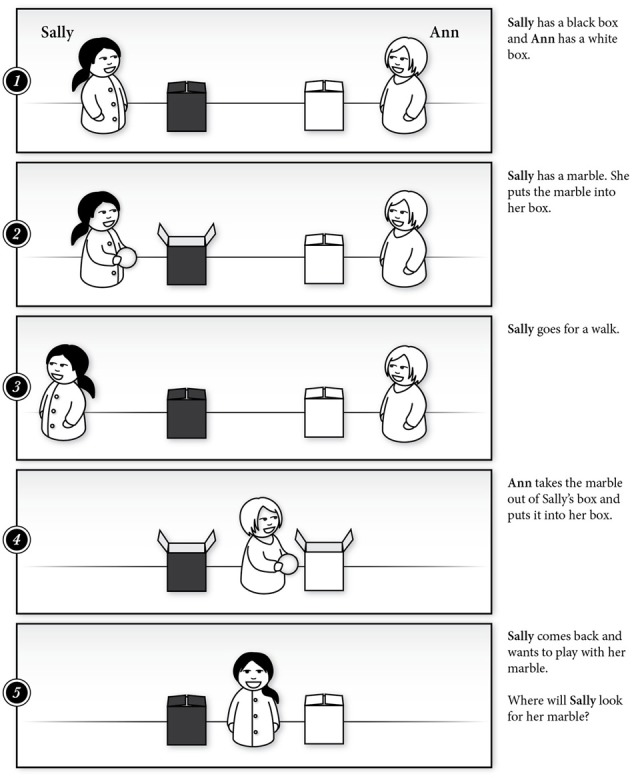
\includegraphics[width=0.4\textwidth]{figures/false_belief_story.jpg}
\caption{False Belief Example \cite{Wimmer_1983}}
\label{fig:falseBelief}
\end{center}
\end{figure}
Social cues are another important phenomenon to observe mental state changes. Those cues are usually referred to as gaze, facial expression, vocal changes, etc{cite}. While gaze cues are more focused on attention, facial/vocal recognition is related to determining the emotional state of others. 



\subsection{Language Model} \label{introLM}
Since the spark of linguistics, researchers try to model language in a scientific fashion by structural (as described in \ref{introLanguage}) or statistical analysis. In the early day of linguistics which solely relies on hard-crafted rules parsing that was purely symbolic\cite{Nadkarni_2011}. When the time came to the digital age, the use of computers largely influenced research, especially in the power to handle huge textual data and the use of machine learning methods which give rise to natural language processing(NLP) for using computers to process human language.

In the domain of NLP, it can be subdivided into 2 main categories, natural language understanding(NLU) and natural language generation(NLG). In the simplest form, NLU can be understood as it performs syntactic and semantic analysis based on the contents in order to classify the meaning of the given text input. NLG on the other hand, is the process of generating text that meets some specific requirement with a given input and condition, for example, text translation. 
 
In order to handle textual data before modeling(NLU or NLG), the data have to go through several numbers of pre-processing  before feeding to any models. Those steps can be summarized in the following\cite{Vijayarani_2015}:
        
        \begin{itemize}
            \item Tokenization
            \item Stop word removal 
            \item Stemming / Lemmatization - 
            \item Embedding - 
        \end{itemize}

\subsubsection{Tokenization}
In English Textual data, it usually comes in paragraph format and needs to break down into atomic levels which  can be done down to individual character levels, but the usual way will be chopping into words as tokens. However, there are problems arise in chopping at the word level which is mostly related to short-form writing style and punctuation, for example: isn't, O'Neil, while it is relatively easy to handle with the case on O'Neil(change to O Neil ), short-form need to be handle in care. It is also reminded that tokenization is language specific where the strategy change with respect to language.

\subsubsection{Stop word Removal}
The tokenization process will generate a huge amount of tokens from the text data, but some of the tokens occur very frequently which may not contribute any meaning to the text itself. Removing those tokens will help in reducing the dimension of word space. There are several methods to determine stop words, for example, pre-defined list, term frequency, inverse document frequency, etc.

\subsubsection{Stemming/Lemmatization}
English words can exist in different forms like initial, initialed, initialing, and initialization which all refer to the root initial. Stemming is the process to identify the root of the token and aims to reduce the inflectional form in order to reduce  the size of tokens. The purpose of lemmatization is the same, but with different methodologies which use vocabulary and morphological analysis of words to apply the transformation while Stemming is more rely on a heuristic process to truncate part of the word.

\subsubsection{Embedding}
Tokens are still in textual format after those processes, however, most language models work on numerical space rather than discrete text space, the embedding process is to transform tokens into numerical form as a final step before input to the model. There are varieties of ways to achieve the purpose, the simplest one will be one-hot encoding which turns each token into a binary array with length equal to the size of tokens. The disadvantage of this is it creates a very high dimension and  sparsity matrix to represent tokens which may impact the model's convergence time and performance. Other's methods include bag of words together with term frequency-inverse document frequency(TF-IDF) to assign a numerical value for tokens. However, the trend changed to use Word2Vec after adopting the neural network which uses the vector representation before the output layer as the token's embedding. The task of the neural network can be either using surrounding context(words) to predict the target word or the opposite way. This way, it heavily reduces the embedding dimension in comparison to the one hot-encoding and uses the surrounding context to assign numerical meaning to tokens.\\
 
During the pre-deep learning era, there is a wide range of modeling such as support vector machine(SVM) that is based on statistical aspects, but the accuracy heavily depends on the data and the prior belief on the kernel selection. After the deep learning era, especially after the invention of the Long-short term memory model (LSTM, an expansion of recurrent neural network RNN) and Transformer (BERT) which change the trend from statistical to auto-regressive model.  The main difference between the two is that RNN-type models are equipped with state space learning\cite{Siegelmann_1995} to enrich the representation of data. \\

In neural network model setup, those pre-processed data are fed into the model in sequential order, and depending on the model's architecture,  the number of tokens (words) input variate, for example, BERT usually will take a predefined maximum input length of the text while LSTM can be done in sliding window which takes a sequence of text at a time. The output will be the classification result base on the input sequence and it learns by calculating the loss between the ground truth label and its result.

\newpage
\section{ToM and Language - Literature Survey} 
From the introduction, it is shown that language(I-language) and ToM is strongly coupled in Linguistics and psychology but has different aspects of external language. Linguistics model E-language as data generated from internal, treating internal language as deep structural(or grammar) that is universal to everyone, but psychology is more focused on how \textbf{external language is affecting the development of the mental state}. There is no doubt that language does matter in mental thought, but the question is what's \textbf{the role of language in building up cognitive structures and their uniqueness in that role\cite{Astington_2005}.} The investigation of the roles of language in ToM can be summarized into four main focuses\cite{Astington_2005}:
\begin{enumerate}
    \item No role at all
    \item Conversational Pragmatics
    \item Lexical Semantics
    \item Complementation Syntax
    \item Synergy (Combine action)
\end{enumerate}
While the no role at all suggested that language is only a tool to access and implement the abstract human mind, others give support that language is crucial to the development of ToM in the form of interaction between the surrounding environment during the infant and pre-school age. All those roles for language are conversational based and each of them provides an explanation of how language helps in build-up ToM, for example, conversational pragmatics suggests language as information exchange promotes the understanding of there are different thoughts by others on the same fact, while lexical semantics and complementation syntax are emphasizing the role of language in formulations of abstract concept from lexical mental verb(e.g happy, sad) and sentential complement.

While the above paragraph describes the relationship between language and ToM in a constructive way, much developmental psychology research provides both correlation and training study in order to show the importance of language. Those studies are primarily focusing on false-beliefs understanding ability as it reveals both internal and external beliefs at the same time. In correlation studies, different age groups of children are examined on both false-belief tasks and language testing to identify the relationship between language capability and the performance of ToM\cite{Ebert_2020}. On the other hand, training study is done by giving variate language training to children and looking for performance differences given by the training. Those training usually variate in the use of words, for example, with or without restriction on the usage of mental verbs (e.g. think, know) and absence of sentential complement sentences\cite{Lohmann_2003}. One of the research\cite{Pyers_2009} takes a step further to investigate language in other forms \- Sign language that is used by deaf people which results in the same conclusion.
 
The research above suggests a strong correlation and the importance of language in the role of ToM development, especially when there is defective during language acquisition, it heavily affects the mental state of understanding in all forms of language.

\section{Language Model - Literature Survey} 
The rise of ChatGPT is storming the world over the past year and it still influencing the world heavily in a wide range of areas. On the research aspect, there is no solid theory that can explain the behavior of those LLM, especially on the generality across different domains of knowledge by simple language training\cite{Bubeck_2023}. The study on\cite{Bubeck_2023} gives a details study on the intelligent ability of LLM and the research on \cite{Kosinski_2023} shows that GPT3.5 solved 90\% of false belief tasks that reached the performance of a seven years old child, it further hypothesized the result of the large language model is attributed to the internal development of ToM as a by-product from solely language training. This hypothesis matches perfectly with the above discussion on the relationship between language and ToM. 
The basic architecture nowadays for language models is dominated by the transformer which composite of an autoencoder and attention mechanism together, without the recurrent unit involved{cite}. However, the positional information is important in language, it is pushed into the embedding as an extracted feature of tokens to represent the sequential order within the text. The main idea of the transformer is to encode the information from input text by the composition of transformation(attention) which result in a complex hidden space for the decoder to perform the relevant tasks such as predicting a missing word in a sentence or the next word generation{cite}. Since the composition of attention is formed recursively by pairs of pair of words, it forms a hierarchical structure of measurement that reproduce the property of maximum mean discrepancy used in measuring the difference between distribution from their samples{cite} and it usually comes with several attention stacks together to form multi-head attention, which it can be thought of capturing different statistical property from the input data. 
But the question of the number of attention needed and the efficiency of increasing attention remains unanswered{cite}. 
It is shown that transformer architecture mainly benefits from the attention mechanism which has its own place in statistics but is this statistical property gives rise to such high accuracy or even the enlightenment of ToM still remains unclear.

\newpage


\section{Experiment Setting} 

\subsection{Data Set and Pre-processing}
The experiment is conducted on the IMDB movie review data set {cite} for sentiment classification. The whole data set consists of 50,000 textual reviews and a target label indicating  positive and negative feedback on the movie. 15,000 reviews are sampled from the data as the training set and 3,000 for testing data. The following table(\ref{tab:dataset}) summarizes the positive and negative class distribution on both the training and test set.
\begin{table}[!h]
    \centering
        \begin{tabular}{||c|c| c||} 
        \hline
 Train/Test & Number of Review & Percentage(Pos / Neg) \\ 
 \hline\hline
 Train  &  15000  & 50\% / 50\% \\ 
 \hline
  Test & 3000  & 50\% / 50\%  \\ 
 \hline
    \end{tabular}
     \caption{Training, Testing Set}
    \label{tab:dataset}
\end{table} 

Those data sets then go through data cleaning(remove html related tags) and pre-processing pipeline as described in \ref{introLM} apart from the last two processes (Stemming/Lemmatization, embedding). The average token count for each review is 105 (=1,581,851/15,000). \\

Since the experiment is conducted on destroying the language, the part of speech(POS) tags are used as a selector to control which part of the text should work on instead of doing it at the token level. The following table(\ref{tab:poscount}) shows the top 10 POS tags count and the corresponding percentage  for the pre-processed data set.

\begin{table}[!h]
\begin{center}
\fontsize{9pt}{9pt}\selectfont
\begin{tabular}{|c|r|c|c|}
\hline
\multicolumn{1}{|l|}{Data Set} & POS tag & Positive review & Negative Review \\ \hline
\multirow{10}{*}{Train}        & NOUN    & 352,846(22.3\%) & 336,466(21.2\%) \\ \cline{2-4} 
                               & VERB    & 165,504(10.4\%)& 167,988(10.6\%) \\ \cline{2-4} 
                               & ADJ     & 140,768(8.8\%) & 133,559(8.4\%)  \\ \cline{2-4} 
                               & PROPN   & 86,150(5.4\%)   & 60,792(3.8\%)  \\ \cline{2-4} 
                               & ADV     & 37,888(2.3\%)   & 40,703(2.5\%)  \\ \cline{2-4} 
                               & NUM     & 10,036(0.6\%)   & 10,977(0.6\%)  \\ \cline{2-4} 
                               & ADP     & 4,911           & 5,620           \\ \cline{2-4} 
                               & DET     & 2,429           & 2,300           \\ \cline{2-4} 
                               & INTJ    & 2,021           & 3,435           \\ \cline{2-4} 
                               & X       & 2,008           & 2,292           \\ \hline
\multirow{10}{*}{Test}         & NOUN    & 74,954          & 69,862          \\ \cline{2-4} 
                               & VERB    & 32,464          & 32,254          \\ \cline{2-4} 
                               & ADJ     & 31,073          & 29,371          \\ \cline{2-4} 
                               & PROPN   & 16,473          & 11,732          \\ \cline{2-4} 
                               & ADV     & 7,580           & 7,715           \\ \cline{2-4} 
                               & DET     & 2,069           & 2,005           \\ \cline{2-4} 
                               & NUM     & 1,870           & 2,073           \\ \cline{2-4} 
                               & ADP     & 937             & 1,146           \\ \cline{2-4} 
                               & INTJ    & 359             & 635             \\ \cline{2-4} 
                               & X       & 344             & 433             \\ \hline
\end{tabular}
     \caption{POS tag count}
    \label{tab:poscount}
\end{center}
\end{table}

\subsection{Simulate Incomplete Language Learning} \label{incomplearning}
The experiment result from developmental psychology suggested a strong correlation between deficiency in language and ToM. The simplest way to simulate the lack of certain types of words in the language is to skip those in the data set, however, it is not appropriate as those psychology experiments avoid using some type of words, but it didn't change the underline meaning of the sentence.    
In order to reflect this scenario in the language model, this experiment proposes 2 methods that try to approximate language deficiency, "always wrong" and Merge. 

\subsubsection{Always Wrong}
The idea behind the method "always wrong" is to trick the model's classification during training at a specific position of the text, since the model is using the output of LSTM for classification, so there is a one-to-one mapping between the result and input token. In this experiment, the position is appointed using POS tag, for example, treat all predictions for ADJ as wrong. The illusion is done by changing the loss value at the corresponding location to 0.5 for the cross-entropy loss function. The purpose of it is to destroy the learning and reflect it has difficulty in understanding the token at that position. Figure(\ref{fig:alwayswrong}) shows briefly how the method works, detail of the full model can be found in \ref{modelarch}.
\begin{figure} [!h]
\begin{center}
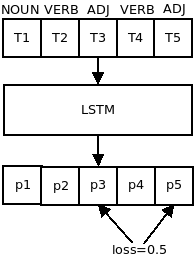
\includegraphics[width=0.2\textwidth]{figures/alwayswrong.png}
\caption{Trick the model on ADJ}
\label{fig:alwayswrong}
\end{center}
\end{figure}

\subsubsection{Token Merge} \label{incompmerge}
The concept of merge tokens origin from the MERGE operator(\ref{introLanguage}) of bare phrase structures, as introduced above, MERGE help to build a structural description set from sentences and assume to take 2 input. This experiment, it is trying to simulate the MERGE in 3 strategies:
\begin{center}
\begin{enumerate}
    \item Random Merge
    \item Merge surrounding words of a specific position
    \item Merge specific POS pattern
\end{enumerate}
\end{center}
Again, the specific position in the second strategy is relying on POS tag, for example, merge tokens that must include ADJ, on the other hand, the third way is to merge tokens in a specific ordered pattern such as ADJ+NOUN. Since it is known that there are common phrases that use in the English language grammar(ex. NOUN phrase), the merge action here is aimed to destroy that structure before it feeds to the model. The details of the merge will be described in \ref{modelMerge}, and the figure(\ref{fig:3waysonmerge}) below shows an example for each strategy.

\begin{figure} [!h]
\begin{center}
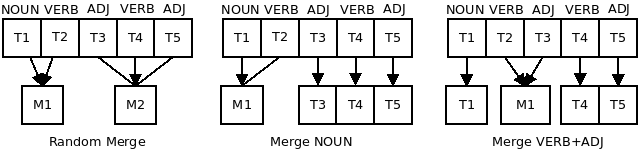
\includegraphics[width=0.7\textwidth]{figures/merge.png}
\caption{3 ways to Merge}
\label{fig:3waysonmerge}
\end{center}
\end{figure}


\subsection{Model Architecture and Training}\label{modelarch}
The architecture for the model consists of 4 main blocks which are Embedding, Merge, LSTM, and classification. The following table(\ref{tab:modelsettings}) and diagram(\ref{fig:modelArch}) give a summary of the parameters set for each block and visualization for the model:
\begin{table}[!h]
\begin{tabular}{|c|l|}
\hline
Block                   & \multicolumn{1}{c|}{Parameters}                                 \\ \hline
Embedding               & embedding dim=256                                               \\ \hline
Merge(Conv1D)          & kernel=2,stride=1                                               \\ \hline
LSTM                    & input dim=256, hidden dim=256, hidden layer=3, bidirection=True \\ \hline
Classification(Linear) & input dim=256*2 , out dim = 3                                   \\ \hline
\end{tabular}
\caption{Model Settings}
\label{tab:modelsettings}
\end{table}
\newpage
\begin{figure} [!h]
\begin{center}
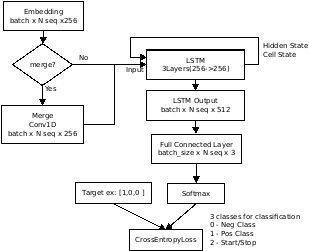
\includegraphics[width=0.6\textwidth]{figures/modelDiagram.png}
\caption{Full model Architecture}
\label{fig:modelArch}
\end{center}
\end{figure}

\subsubsection{Token Merge Block} \label{modelMerge}
As described in \ref{incompmerge}, one of the methods to simulate incomplete language is by merging specific tokens which is done by function prepareMerge(\ref{alg:prepareMerge}) and Conv1D. There are 3 parameters to define for merging: 
\begin{enumerate}
    \item $\alpha$ the minimum token to merge 
    \item $\beta$ the maximum token to merge
    \item $l$ a random merge list of size equal input sequence length, lower and upper clipped by $\alpha,\beta$ (ex: [2,3,3,2,3,2]) 
\end{enumerate}

After tokens pass through the embedding layer, it will result in an embedding tensor($\mathbb{E}$) of size NxE (N=sequence length, E=embedding dim). This matrix will then transform to a merge tensor($\methbb{M}$) of size NxEx$\beta$ by selecting the number of tokens to merge($l[i]$) with padding zero at the back if the number of tokens is smaller than $\beta$. The following code demonstrated how the merge is prepared before feeding to Conv1D.

\SetKwComment{Comment}{//}{}
\begin{algorithm}
\fontsize{7pt}{7pt}\selectfont
\caption{PrepareMerge}\label{alg:prepareMerge}
\begin{algorithmic}
\Comment{E=embedding dim,N=sequence length} 
\KwData{$l = [2,3,3,2,3,2]$}
\KwData{$\mathbb{E} = Embedding(tokens).reshape(E,-1)$ } 
\KwData{$\mathbb{M} = tensor.zero(N,E,\beta)$}

\Comment{Start from the end} 
$y \gets l.length()-1$\\
$c \gets l.length()$\\
\While{$c \neq 0$}{
$\mathbb{T} = tensor.zero(E,\beta)$ \\
$m \gets l[y]$\\
$s \gets (c-m)$\\
$\mathbb{T} = \mathbb{E}[:,s:c]$\\
$\mathbb{M}[y] =\mathbb{T}$\\
$c \gets c-s$\\
$y \gets y-1$

}
\end{algorithmic}
\end{algorithm}

The merge tensor $\mathbb{M}$ will be used as input to Conv1D(k=2,stride=1) so that each slice of $\mathbb{M}$ is transformed to the size of (E,1). The following figure(\ref{fig:prepareMerge}) visualized the size transformation from embedding until merge:
\begin{figure} [!h]
\begin{center}
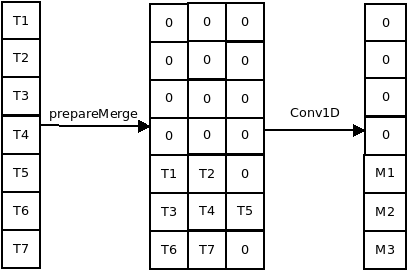
\includegraphics[width=0.3\textwidth]{figures/prepareMerge.png}
\caption{prepareMerge: N=7, $l=[2,2,3,3,2,3,2]$}
\label{fig:prepareMerge}
\end{center}
\end{figure}


\subsubsection{Training}
The review will be fed to the model by pre-defined sequence length and sliding window as a sequence of blocks. The hidden and cell state of LSTM is initialized to 0 at the start of the review and both states of the current block are fed back to the model together with the next block of input(fig.\ref{fig:modeFeedBack}). Thus, the average prediction made for one review is 105. A mini-batch of size 1000 reviews is sampled from the training set as 1 epoch of training, then the test set is fed after each epoch to evaluate the performance of the model. The performance of the model is measured by the average classification result($\hat{\mu}$) of the last 20 tokens sequence, the result is treated as correctly classified if:\\
$abs(\hat{\mu}-targe)<0.05$
   
\begin{figure} [!h]
\begin{center}
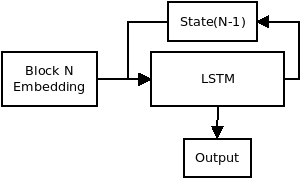
\includegraphics[width=0.3\textwidth]{figures/autoreg.png}
\caption{Feed Back}
\label{fig:modeFeedBack}
\end{center}
\end{figure}
The following tables(\ref{tab:generalsettings},\ref{tab:incompsettings}) summarized the general configuration and the incomplete language training setting for experiment runs.
\begin{table}[!h]
\begin{center}
\begin{tabular}{|c|c|c|c|}
\hline
sequence length & mini-batch size & Optimizator              & Loss function \\ \hline
5,10,25,50,600  & 1000            & Adam(default parameters) & CrossEntropy  \\ \hline
\end{tabular}
\end{center}
\caption{General Settings}
\label{tab:generalsettings}
\end{table}

\begin{table}[!h]
\begin{center}
\begin{tabular}{|l|l|}
\hline
\begin{tabular}[c]{@{}l@{}}Incomplete\\ language Method\end{tabular} & \multicolumn{1}{c|}{POS tag}                                    \\ \hline
Always Wrong                                                         & \multicolumn{1}{c|}{NOUN, VERB, ADJ, ADJ+NOUN, NOUN+VERB+ADJ} \\ \hline
Random Merge                                                         & N/A                                                             \\ \hline
Merge Specific Tags                                                  & NOUN,PROPN,VERB,ADJ,SCONJ,CONJ                                  \\ \hline
Merge Specific Patten                                                & ADJ+NOUN, NOUN+VERB+ADJ,  NOUN+VERB                             \\ \hline
\end{tabular}
\caption{Incomplete Language Setting}
\label{tab:incompsettings}
\end{center}
\end{table}

\newpage
\section{Experiment Result and Discussion} 
In this section, the experiment results of the two incomplete languages setup are presented on the test set. First of all, the base case results  for each sequence length are shown in the following table(\ref{tab:basecaseResult}).

\begin{table}[!h]
\begin{center}
\begin{tabular}{c|ccccc|}
\cline{2-5}
\multicolumn{1}{l|}{}                 & \multicolumn{5}{c|}{Test set Accuracy(\%)}                                                                                         \\ \hline
\multicolumn{1}{|c|}{sequence length} & \multicolumn{1}{c|}{mean}  & \multicolumn{1}{l|}{quartile 25\%} & \multicolumn{1}{l|}{median} & \multicolumn{1}{l|}{quartile 75\%} & \multicolumn{1}{l|}{IQR} \\ \hline
\multicolumn{1}{|c|}{5}               & \multicolumn{1}{c|}{0.66}  & \multicolumn{1}{c|}{0.656}         & \multicolumn{1}{c|}{0.668}  & \multicolumn{1}{c|}{0.679} & 0.023                            \\ \hline
\multicolumn{1}{|c|}{10}              & \multicolumn{1}{c|}{0.681} & \multicolumn{1}{c|}{0.683}         & \multicolumn{1}{c|}{0.701}  & \multicolumn{1}{c|}{0.713} & 0.03                             \\ \hline
\multicolumn{1}{|c|}{25}              & \multicolumn{1}{c|}{0.708} & \multicolumn{1}{c|}{0.730}         & \multicolumn{1}{c|}{0.740}  & \multicolumn{1}{c|}{0.745} & 0.015                            \\ \hline
\multicolumn{1}{|c|}{50}              & \multicolumn{1}{c|}{0.762} & \multicolumn{1}{c|}{0.773}         & \multicolumn{1}{c|}{0.778}  & \multicolumn{1}{c|}{0.781}  & 0.008                            \\ \hline
\multicolumn{1}{|c|}{600}             & \multicolumn{1}{c|}{0.754} & \multicolumn{1}{c|}{0.768}         & \multicolumn{1}{c|}{0.792}  & \multicolumn{1}{c|}{0.801}  &0.033                           \\ \hline
\end{tabular}
\caption{Base Case Result (~450 epochs for 2 runs)}
\label{tab:basecaseResult}
\end{center}
\end{table}
The above base case results show that the mean accuracy is growing together with increasing sequence length of blocks. One thing to notice is that apart from the sequence length of 5, all others' accuracy distribution is left-skewed. The mean accuracy of each sequence length will be used as a baseline to compare the experiment result on those deficiency language training, so, results from onward are \textbf{changed to Ratio Based where the divisor is the mean accuracy of each sequence.} Thus, the interruption of the value from each table below is the \textbf{performance degradation relative to the base case} with 1 representing no changes and 0 means fully degraded.

\subsubsection{Always Wrong Method}
The result of "always wrong" is separated into 2 categories, the first one is to show the result on only 1 POS tag specified while the second one is using more than 1 POS tag. The performance of the model is listed in the following table(\ref{tab:alwayswrongDegrade}), details of result can be found in (\ref{appendix:alwayswrongonly1},\ref{appendix:alwayswrongADJNOUN})  

\begin{table}[!h]
\fontsize{10pt}{10pt}\selectfont
\begin{tabular}{|c|c|c|c|c|}
\hline
seq len & Degrade 1 & Degrade 2 & Degrade 3 & Average Degrade \\ \hline
5       & 1         & 0.97      & 0.95     & 0.97 \\ \hline
10      & 0.96      & 0.96      & 0.94     & 0.95 \\ \hline
25      & 0.96      & 0.98      & 0.98     & 0.97  \\ \hline
50      & 0.95      & 0.94      & 0.97     & 0.95 \\ \hline
\end{tabular}
\caption{Performance Degrade by always wrong. \\
Column 1-(NOUN,VERB, ADJ)\\ 
Column 2-(ADJ \& NOUN)\\
Column 3-Other's}
\label{tab:alwayswrongDegrade}
\end{table}

In general, the above results show that the "always wrong" method doesn't largely impact the performance, \textbf{with an average degradation from 3\% to 5\%}. Especially, with the sequence length of 5, it shows nearly no difference in comparison to the base case. It is also stressed that those are from a disrupted training which in average over 50\% of loss value is modified(table\ref{tab:poscount}). Although the mean accuracy looks good in this experiment, it shows some differences in the distribution once comparing the inter-quartile range(IQR), and the ratio between the base case shown in the following table(\ref{tab:alwayswrongIQR}).   
\begin{table}[!h]
\fontsize{10pt}{10pt}\selectfont
\begin{center}
\begin{tabular}{|c|c|c|c|}
\hline
seq len & (NOUN,VERB,ADJ) & (ADJ \& NOUN) & Other's \\ \hline
5       & 1.6             & 1.4         & 1.4    \\ \hline
10      & 0.7             & 1.13         & 1.13    \\ \hline
25      & 1.26            & 2            & 1.9     \\ \hline
50      & 3.7             & 5.3          & 1.7     \\ \hline
\end{tabular}
\caption{IQR comparison (Ratio) }
\label{tab:alwayswrongIQR}
\end{center}
\end{table}

Those figures suggested that for larger sequences of blocks (ie. >=25), the accuracy distribution is more affected by the method and the most contribution to the change in IQR is by using ADJ and NOUN together.
A control case of always wrong with "NOUN \& VERB \& ADJ \& PROPN \& ADV \& INTJ" is done and the average accuracy is 0.16. 

\subsubsection{Token Merge}
The experiment results on token merge are presented in 2 parts, the first part will focus on the comparison between random merge and merge on POS tag, followed by the second part on presenting the result of merge with a specific pattern. The random merge is done with minimum and maximum merge set to 2 and 3 correspondingly. The result is summarized in the following(\ref{tab:mergeDegrade}):

\begin{table}[!h]
\fontsize{10pt}{10pt}\selectfont
\begin{tabular}{|c|c|c|l|c|l|l|}
\hline
seq len & Random & NOUN & VERB  & ADJ  & CCONJ & SCONJ \\ \hline
5       & 0.893  &      & 0.9   & 0.95 &       &       \\ \hline
10      & 0.88   &      & 0.88  & 0.88 &       &       \\ \hline
25      & 0.87   &      & 0.857 & 0.8  &       &       \\ \hline
50      & 0.88   &      & 0.854 & 0.52 &       &       \\ \hline
\end{tabular}
\caption{Performance Degrade by Random Merge \& POS Tag Merge.}
\label{tab:mergeDegrade}
\end{table}
The result of random merge on all sequences shows roughly the same level of degradation($\approx12\%$). It also noted that in the random merge experiment, \textbf{the merged pattern is different} for short($\leq10$) and long sequences ($\geq25$). The detail on pattern differences and test results are attached in the appendix(\ref{appendix:top10RMergeDiff},\ref{appendix:verbMerge},\ref{appendix:adjMerge}) .\\

While the performance of those shorter sequences seems to be invariant to token merge, it is not the same for longer sequences. The performance degradation is increasing according to \textbf{tag ordering: NOUN, VERB, ADJ}. The relation between degradation, sequence length, and tag is visualized in the following diagram(\ref{fig:mergeScatter}).
\begin{figure} [!h]
\begin{center}
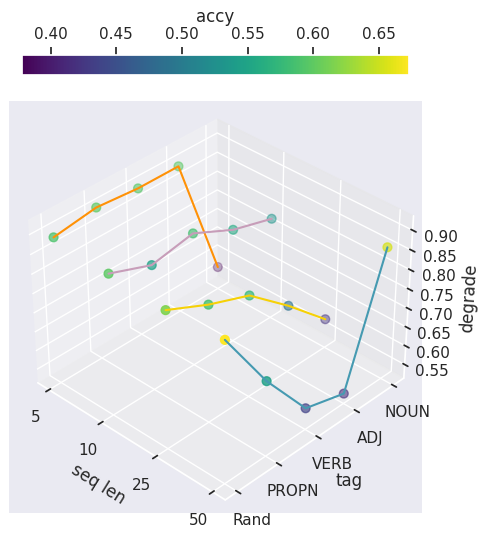
\includegraphics[width=0.4\textwidth]{figures/tokenmerg1.png}
\caption{Token Merger: Degradation vs Sequence len vs Merge Tag}
\label{fig:mergeScatter}
\end{center}
\end{figure}
The comparison of the token merge result suggested that the merge on ADJ is different from others' merge significantly on longer sequences, so, in order to confirm the finding, Wilcoxon signed-rank test is used to test the median accuracy of ADJ is different from others, it is done on the result of 25 sequences length with a sampling data point of 290. 
The test on the null hypothesis which the accuracy median of VERB is the same for ADJ is rejected with p-value $2.05\times10^{-11}$ at 95\% confidence level. On the other hand, the same test is applied for VERB and PROPN, the result shows strong evidence to support the null hypothesis with p-value $0.7$. The details of the statistical test can be found in the appendix(\ref{appendix:signedranktestseq25}). The following figures show the accuracy distribution on each case(\ref{fig:displot1}) 
\begin{figure} [!h] 
\begin{subfigure}[h]{0.3\linewidth} 
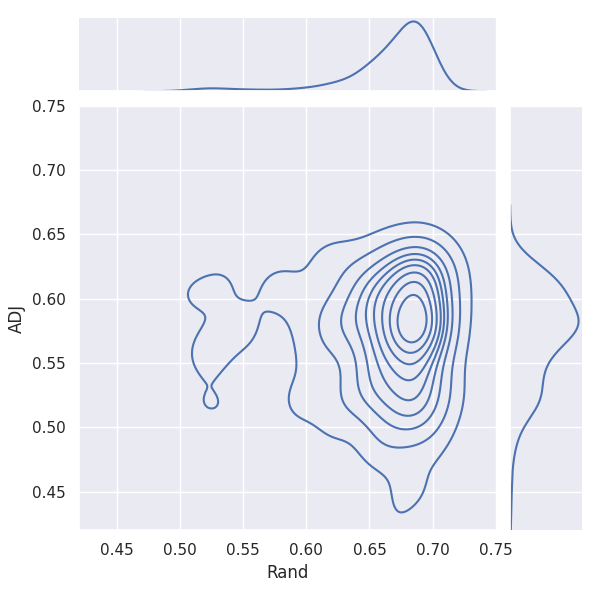
\includegraphics[width=\linewidth]{figures/merge_adj_rand_joinplot.png}
\caption{Join distribution plot on Accuracy\\ADJ \& Random}
\end{subfigure}
\hfill
\begin{subfigure}[h]{0.3\linewidth} 
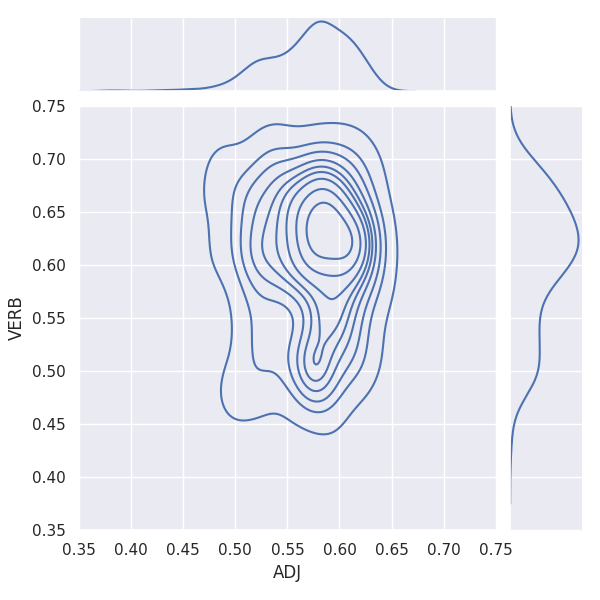
\includegraphics[width=\linewidth]{figures/merge_adj_verb_joinplot.png}
\caption{Join distribution plot on Accuracy\\ADJ \& VERB}
\end{subfigure}
\hfill
\begin{subfigure}[h]{0.3\linewidth}
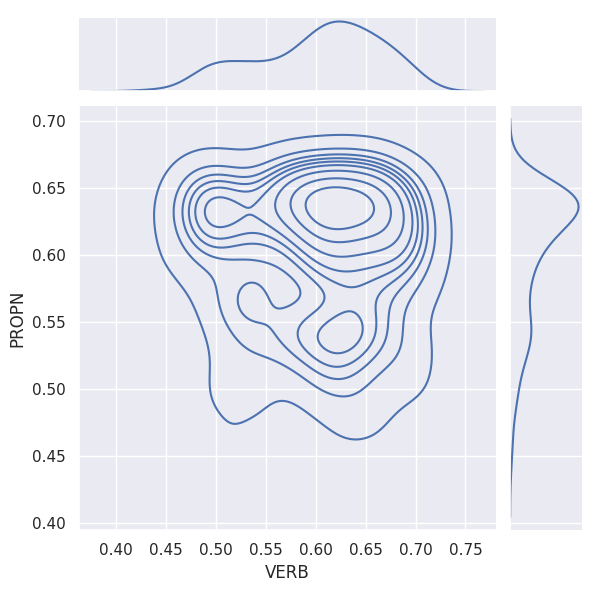
\includegraphics[width=\linewidth]{figures/merge_verb_propn_joinplot.png}
\caption{Join distribution plot on Accuracy\\VERB \& PROPN}
\label{fig:displot1}
\end{subfigure}
\end{figure}
\newpage
The experiments result above suggested that the sequence block size will result in different behavior on the performance degradation, and the block size difference can mainly be separated into shorter($\leq10$) and longer($\geq25$), in a result, the fixed pattern merge will switch to focus on sequence length of 10 and 25 and the finding of different merge pattern (\ref{appendix:top10RMergeDiff}). The patterns that are used are oriented with POS tags ADJ, VERB, and NOUN. The table(\ref{tab:fixmerge1},\ref{tab:fixmerge2}) below gives an overview of the degradation according to different patterns, and the details are placed in the appendix(\ref{appendix:adjnounMerge},\ref{appendix:nounverbadjMerge},\ref{appendix:verbnounMerge}).

\begin{table}[!h]
\fontsize{10pt}{10pt}\selectfont
\begin{tabular}{|c|c|c|c|}
\hline
seq len & \begin{tabular}[c]{@{}c@{}}attributeive adjectives\\ Adj+Noun\end{tabular} & \begin{tabular}[c]{@{}c@{}}predicative adjective\\ Verb+Adj\end{tabular} & \begin{tabular}[c]{@{}c@{}}postpositive adjective\\ Noun+Adj\end{tabular} \\ \hline
10      & 0.833                                                                      &                                                                          &                                                                           \\ \hline
25      & 0.549                                                                      &                                                                          &                                                                           \\ \hline
\end{tabular}
\caption{Merge fixed pattern(1)}
\label{tab:fixmerge1}
\end{table}

\begin{table}[!h]
\fontsize{10pt}{10pt}\selectfont
\begin{tabular}{|c|c|c|c|l|}
\hline
seq len & \begin{tabular}[c]{@{}c@{}}Object\\ Verb+Noun\end{tabular} & \begin{tabular}[c]{@{}c@{}}Subject\\ Noun+Verb\end{tabular} & Adj+Verb & Noun+Verb+Adj \\ \hline
10      & 0.698                                                       &                                                            &          & 0.786         \\ \hline
25      & 0.549                                                       &                                                            &          & 0.646         \\ \hline
\end{tabular}
\caption{Merge fixed pattern(2)}
\label{tab:fixmerge2}
\end{table}

The result above indicates that the sequence length of 25 on all fixed pattern merges can only achieve $50\%\sim60\%$ of the base case performance and those are already under $0.5$ accuracy which means it fails to learn at all. In contrast to the short sequences which still maintain over $70\%$ performance relative to the base case on some pattern(ADJ+NOUN, NOUN+ADJ+VERB), but also notice that the accuracy is just slightly over $0.5$.

One thing to notice is that the shorter sequence length shows the ability to influence on fixed pattern ADJ+NOUN but not for the longer block which may suggest the structure they acquired may be different. In addition, the shorter and longer sequence of input can be thought of as simulating the sensory-motor aspect\cite{Hauser_2002} on reading capability. 


\clearpage
\section{Conclusion}

The above experiments have demonstrated two different methods that try to degrade the performance of a small language model in semantics classification. While the result of the "always wrong" method shows little effect on the performance of the model, it also raises the question of why from the statistical point of view as the training is heavily disturbed. \\

One may argue that it is unclear on the token distribution of positive and negative classes so those tags that are tested are not right on the target. But the point of using POS tag is to avoid this problem. The idea is to treat the data as an observational study and use POS tag as an instrumental variable(IV) (fig\ref{fig:combinIV} upper path). In this way, the treatment will be a normal token when it is off(not in the list of tags) or disturb token when it is on. Moreover, either positive or negative related tokens are grouped under part of speech, for example, "good" or "bad" in adjectives, so that the disturb on learning is applied in a fair sense. \\

Another though from the statistical side is that, from the observation on the embedding weight that doesn't change much from initial(\ref{context:embeddoesntchange})

The interpretation with IV suggested that the effect of tokens with respect to POS Tag partition has a small effect on the outcome and gives supporting evidence to the belief that the learning of semantics classification is not limited to statistics. 
\begin{figure} [!h]
\begin{center}
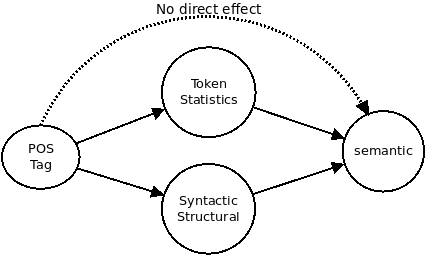
\includegraphics[width=0.6\textwidth]{figures/combin_IV.png}
\caption{Instrumental Variable Hypothesis}
\label{fig:combinIV}
\end{center}
\end{figure}

In addition to the finding above, the test on toke merge further suggested that structural plays an important role in inferring semantics from the language with the same argument on IV. The merge operation destroys the original structure before feeding for modeling and the different effect caused by it support the hypothesis. 

However, it may criticize that apart from the structure, the merge also destroys the representation of the token and try to merge non-sense word together. It is admitted that those questions are not easy to answer and require more research and experiments, but yet, there are some findings that can be shared in order to prepare a deeper investigation. First of all, it is observed that the weight distribution of the embedding layer doesn't change much\label{context:embeddoesntchange} in both the base case and merge(fig\ref{fig:modelWeight}). This shows that in end-to-end training on classification, the embedding of a token doesn't work like those word2Vec methods which try to assign a token's representation by surrounding tokens and all it needs is a unique representation. Thus, from that point of view, token representation reduces to symbolic representation without any project of human meaning on the numerical value. On the other hand, the inspection of the weight of the merge block(Conv1D) also suggested that the layer does learn since the distribution of weight is changed heavily from the normal distribution that centers around zero to a much more flattened distribution(fig\ref{fig:modelWeight}). But the question of what it learns still remains in mystery. \\
\begin{figure} [!h] 
\begin{subfigure}[h]{0.3\linewidth} 
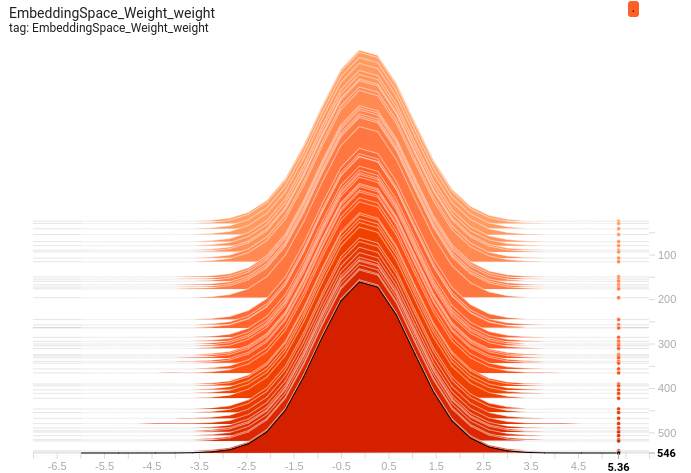
\includegraphics[width=\linewidth]{figures/RandMerge_Seq25EmbeddingWeight.png}
\caption{Random Merge - seq25 Embedding Weight}
\end{subfigure}
\hfill
\begin{subfigure}[h]{0.3\linewidth} 
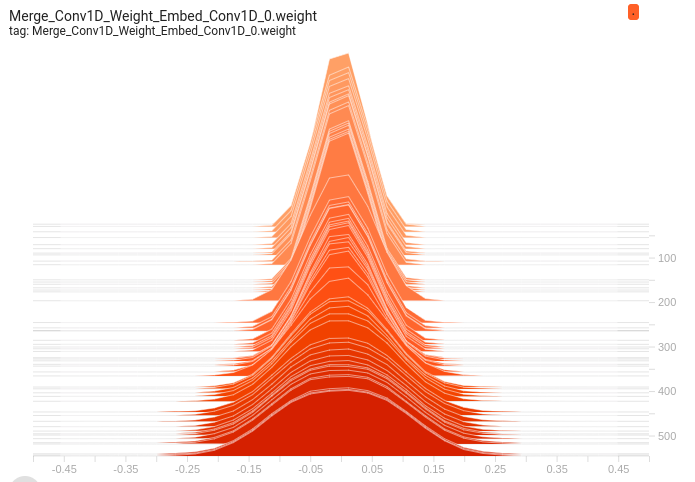
\includegraphics[width=\linewidth]{figures/RandMerge_seq25_conv1d_1.png}
\caption{Random Merge - seq25 Conv1D\_1 Weight}
\end{subfigure}
\hfill
\begin{subfigure}[h]{0.3\linewidth}
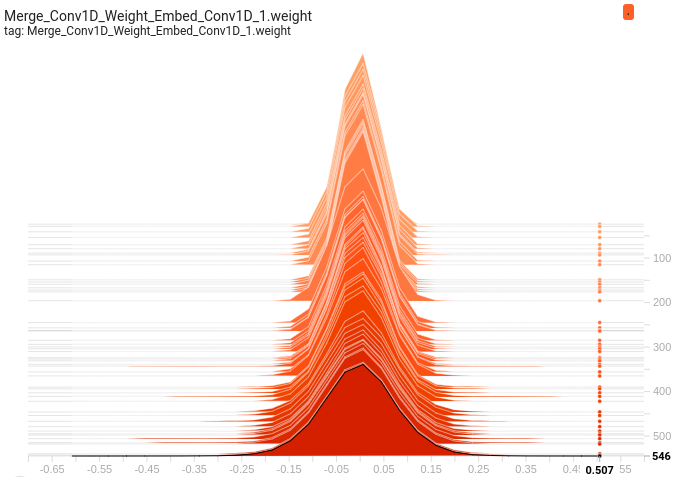
\includegraphics[width=\linewidth]{figures/RandMerg_seq25_conv1d_2.png}
\caption{Random Merge - seq25 Conv1D\_2 Weight}
\label{fig:modelWeight}
\end{subfigure}
\end{figure}

This thesis gives preliminary insight into how inference on the mental state by language model may be affected in a very small setting, both on the class to infer(just 2 classes) and model architecture. The result may be very different if the state to infer is increased. Furthermore, the effect on merge and the different behavior on random and fixed pattern merge is questionable on why the random case is still able to learn but not for the fixed one. In addition, the truth behind the structure is still unclear, as it can be in a syntactic form(tree base), computational state(automata), a combination of the two, or other types of structures. Last but not least, the interaction between natural language understanding and generation is still a missing puzzle in the study of the language model and it is hoped that this research on how internal language may influence by external language initial a tiny step in this direction.

\newpage






\newpage

% BibTeX bibliography
\bibliographystyle{alpha} %plain=[1], alpha=[BGZ09]
\bibliography{Thesis_ref}

\addcontentsline{toc}{section}{\refname}


% Use Biblatex if you have problems with Estonian keywords
%\printbibliography %biblatex


% Use alternative local LaTeX bibliography
\begin{comment}
\begin{thebibliography}{9}
\bibitem{proVerif} 
  Bruno Blanchet. 
  Proverif: Cryptographic protocol verifier in the formal model.
  \url{http://www.proverif.ens.fr/}.
  (checked 15.05.2012)
\bibitem{GameB_1} GameB1
\bibitem{GameB_2} GameB2
\bibitem{certicrypt} certicrypt
\bibitem{kamm12} kamm12
\end{thebibliography}
\end{comment}


\newpage
%\appendix
%\section*{\appendixname}
\iflanguage{english}%
  {\section*{Appendix}
  \addcontentsline{toc}{section}{Appendix}
  }%
  {\section*{Lisad}
  \addcontentsline{toc}{section}{Lisad}}


\section*{I. Glossary}
\addcontentsline{toc}{subsection}{I. Glossary}
\begin{table}[!h]
\begin{tabular}{c|ccccc|}
\cline{2-6}
\multicolumn{1}{l|}{}         & \multicolumn{5}{c|}{Test Set Accuracy \% (NOUN,VERB,ADJ)}                                                                                                     \\ \hline
\multicolumn{1}{|c|}{seq len} & \multicolumn{1}{c|}{mean}  & \multicolumn{1}{c|}{quartile 25\%} & \multicolumn{1}{l|}{median} & \multicolumn{1}{l|}{quartile 75\%} & \multicolumn{1}{l|}{IQR} \\ \hline
\multicolumn{1}{|c|}{5}       & \multicolumn{1}{c|}{0.66}  & \multicolumn{1}{c|}{0.65}          & \multicolumn{1}{c|}{0.679}  & \multicolumn{1}{c|}{0.692}         & 0.042                    \\ \hline
\multicolumn{1}{|c|}{10}      & \multicolumn{1}{c|}{0.66}  & \multicolumn{1}{c|}{0.669}         & \multicolumn{1}{c|}{0.68}   & \multicolumn{1}{c|}{0.69}          & 0.021                    \\ \hline
\multicolumn{1}{|c|}{25}      & \multicolumn{1}{c|}{0.681} & \multicolumn{1}{c|}{0.711}         & \multicolumn{1}{c|}{0.725}  & \multicolumn{1}{c|}{0.730}         & 0.019                    \\ \hline
\multicolumn{1}{|c|}{50}      & \multicolumn{1}{c|}{0.727} & \multicolumn{1}{c|}{0.729}         & \multicolumn{1}{c|}{0.761}  & \multicolumn{1}{c|}{0.766}         & 0.037                    \\ \hline
\end{tabular}
\caption{Test Accuracy Details on Always Wrong with only 1 POS Tag.}
\label{appendix:alwayswrongonly1}
\end{table}

\begin{table}[!h]
\begin{tabular}{c|ccccc|}
\cline{2-6}
\multicolumn{1}{l|}{}         & \multicolumn{5}{c|}{Test Set Accuracy \% (ADJ+NOUN)}                                                                                       \\ \hline
\multicolumn{1}{|c|}{seq len} & \multicolumn{1}{c|}{mean}  & \multicolumn{1}{c|}{quartile 25\%} & \multicolumn{1}{c|}{median} & \multicolumn{1}{c|}{quartile 75\%} & IQR   \\ \hline
\multicolumn{1}{|c|}{5}       & \multicolumn{1}{c|}{0.642} & \multicolumn{1}{c|}{0.637}         & \multicolumn{1}{c|}{0.657}  & \multicolumn{1}{c|}{0.669}         & 0.032 \\ \hline
\multicolumn{1}{|c|}{10}      & \multicolumn{1}{c|}{0.654} & \multicolumn{1}{c|}{0.651}         & \multicolumn{1}{c|}{0.675}  & \multicolumn{1}{c|}{0.685}         & 0.034 \\ \hline
\multicolumn{1}{|c|}{25}      & \multicolumn{1}{c|}{0.699} & \multicolumn{1}{c|}{0.701}         & \multicolumn{1}{c|}{0.719}  & \multicolumn{1}{c|}{0.731}         & 0.03  \\ \hline
\multicolumn{1}{|c|}{50}      & \multicolumn{1}{c|}{0.722} & \multicolumn{1}{c|}{0.717}         & \multicolumn{1}{c|}{0.765}  & \multicolumn{1}{c|}{0.771}         & 0.053 \\ \hline
\end{tabular}
\caption{Test Accuracy Details on Always Wrong with ADJ & NOUN .}
\label{appendix:alwayswrongADJNOUN}
\end{table}

\begin{table}[!h]
\begin{tabular}{c|ccccc|}
\cline{2-6}
\multicolumn{1}{l|}{}         & \multicolumn{5}{c|}{Test Set Accuracy \% (Others)}                                                                                         \\ \hline
\multicolumn{1}{|c|}{seq len} & \multicolumn{1}{c|}{mean}  & \multicolumn{1}{c|}{quartile 25\%} & \multicolumn{1}{c|}{median} & \multicolumn{1}{c|}{quartile 75\%} & IQR   \\ \hline
\multicolumn{1}{|c|}{5}       & \multicolumn{1}{c|}{0.66}  & \multicolumn{1}{c|}{0.655}         & \multicolumn{1}{c|}{0.676}  & \multicolumn{1}{c|}{0.687}         & 0.032 \\ \hline
\multicolumn{1}{|c|}{10}      & \multicolumn{1}{c|}{0.654} & \multicolumn{1}{c|}{0.651}         & \multicolumn{1}{c|}{0.675}  & \multicolumn{1}{c|}{0.685}         & 0.034 \\ \hline
\multicolumn{1}{|c|}{25}      & \multicolumn{1}{c|}{0.699} & \multicolumn{1}{c|}{0.702}         & \multicolumn{1}{c|}{0.722}  & \multicolumn{1}{c|}{0.731}         & 0.029 \\ \hline
\multicolumn{1}{|c|}{50}      & \multicolumn{1}{c|}{0.744} & \multicolumn{1}{c|}{0.754}         & \multicolumn{1}{c|}{0.768}  & \multicolumn{1}{c|}{0.771}         & 0.017 \\ \hline
\end{tabular}
\caption{Test Accuracy Details on Always Wrong (Others) .}
\label{appendix:alwayswrongOthers}
\end{table}


\begin{table}[!h]
\begin{tabular}{c|ccccc|}
\cline{2-6}
\multicolumn{1}{l|}{}         & \multicolumn{5}{c|}{Test Set Accuracy \% (Random)}                                                                                         \\ \hline
\multicolumn{1}{|c|}{seq len} & \multicolumn{1}{c|}{mean}  & \multicolumn{1}{c|}{quartile 25\%} & \multicolumn{1}{c|}{median} & \multicolumn{1}{c|}{quartile 75\%} & IQR   \\ \hline
\multicolumn{1}{|c|}{5}       & \multicolumn{1}{c|}{0.589} & \multicolumn{1}{c|}{0.548}         & \multicolumn{1}{c|}{0.605}  & \multicolumn{1}{c|}{0.642}         & 0.094 \\ \hline
\multicolumn{1}{|c|}{10}      & \multicolumn{1}{c|}{0.599} & \multicolumn{1}{c|}{0.572}         & \multicolumn{1}{c|}{0.606}  & \multicolumn{1}{c|}{0.637}         & 0.065 \\ \hline
\multicolumn{1}{|c|}{25}      & \multicolumn{1}{c|}{0.616} & \multicolumn{1}{c|}{0.594}         & \multicolumn{1}{c|}{0.637}  & \multicolumn{1}{c|}{0.655}         & 0.061 \\ \hline
\multicolumn{1}{|c|}{50}      & \multicolumn{1}{c|}{0.673} & \multicolumn{1}{c|}{0.669}         & \multicolumn{1}{c|}{0.694}  & \multicolumn{1}{c|}{0.705}         & 0.036 \\ \hline
\end{tabular}
\caption{Test Accuracy Details on Random Merge .}
\label{appendix:randMerge}
\end{table}


\begin{table}[!h]
\begin{tabular}{c|ccccc|}
\cline{2-6}
\multicolumn{1}{l|}{}         & \multicolumn{5}{c|}{Test Set Accuracy \% (VERB)}                                                                                           \\ \hline
\multicolumn{1}{|c|}{seq len} & \multicolumn{1}{c|}{mean}  & \multicolumn{1}{c|}{quartile 25\%} & \multicolumn{1}{c|}{median} & \multicolumn{1}{c|}{quartile 75\%} & IQR   \\ \hline
\multicolumn{1}{|c|}{5}       & \multicolumn{1}{c|}{0.595} & \multicolumn{1}{c|}{0.566}         & \multicolumn{1}{c|}{0.612}  & \multicolumn{1}{c|}{0.630}         & 0.064 \\ \hline
\multicolumn{1}{|c|}{10}      & \multicolumn{1}{c|}{0.602} & \multicolumn{1}{c|}{0.592}         & \multicolumn{1}{c|}{0.634}  & \multicolumn{1}{c|}{0.653}         & 0.061 \\ \hline
\multicolumn{1}{|c|}{25}      & \multicolumn{1}{c|}{0.607} & \multicolumn{1}{c|}{0.568}         & \multicolumn{1}{c|}{0.616}  & \multicolumn{1}{c|}{0.649}         & 0.081 \\ \hline
\multicolumn{1}{|c|}{50}      & \multicolumn{1}{c|}{0.651} & \multicolumn{1}{c|}{0.638}         & \multicolumn{1}{c|}{0.671}  & \multicolumn{1}{c|}{0.685}         & 0.047 \\ \hline
\end{tabular}
\caption{Test Accuracy Details on Merge with VERB .}
\label{appendix:verbMerge}
\end{table}

\begin{table}[!h]
\begin{tabular}{c|ccccc|}
\cline{2-6}
\multicolumn{1}{l|}{}         & \multicolumn{5}{c|}{Test Set Accuracy \% (ADJ)}                                                                                            \\ \hline
\multicolumn{1}{|c|}{seq len} & \multicolumn{1}{c|}{mean}  & \multicolumn{1}{c|}{quartile 25\%} & \multicolumn{1}{c|}{median} & \multicolumn{1}{c|}{quartile 75\%} & IQR   \\ \hline
\multicolumn{1}{|c|}{5}       & \multicolumn{1}{c|}{0.597} & \multicolumn{1}{c|}{0.575}         & \multicolumn{1}{c|}{0.608}  & \multicolumn{1}{c|}{0.634}         & 0.059 \\ \hline
\multicolumn{1}{|c|}{10}      & \multicolumn{1}{c|}{0.605} & \multicolumn{1}{c|}{0.588}         & \multicolumn{1}{c|}{0.612}  & \multicolumn{1}{c|}{0.629}         & 0.041 \\ \hline
\multicolumn{1}{|c|}{25}      & \multicolumn{1}{c|}{0.567} & \multicolumn{1}{c|}{0.544}         & \multicolumn{1}{c|}{0.575}  & \multicolumn{1}{c|}{0.596}         & 0.052 \\ \hline
\multicolumn{1}{|c|}{50}      & \multicolumn{1}{c|}{0.398} & \multicolumn{1}{c|}{0.349}         & \multicolumn{1}{c|}{0.487}  & \multicolumn{1}{c|}{0.490}         & 0.141 \\ \hline
\end{tabular}
\caption{Test Accuracy Details on Merge with ADJ.}
\label{appendix:adjMerge}
\end{table}

\begin{table}[!h]
\begin{center}
\fontsize{10pt}{10pt}\selectfont
\begin{tabular}{|ll|}
\hline
\multicolumn{2}{|c|}{Top 10 Merge Pattern}                      \\ \hline
\multicolumn{1}{|c|}{$\leq10$}            & \multicolumn{1}{c|}{$\geq25$} \\ \hline
\multicolumn{1}{|l|}{NOUN\_NOUN}      & ADJ\_ADJ\_ADJ              \\ \hline
\multicolumn{1}{|l|}{ADJ\_NOUN}       & ADJ\_ADJ                  \\ \hline
\multicolumn{1}{|l|}{NOUN\_VERB}      & NOUN\_NOUN                \\ \hline
\multicolumn{1}{|l|}{VERB\_NOUN}      & ADJ\_NOUN                 \\ \hline
\multicolumn{1}{|l|}{NOUN\_NOUN\_NOUN} & NOUN\_VERB                \\ \hline
\multicolumn{1}{|l|}{ADJ\_ADJ}        & VERB\_NOUN                \\ \hline
\multicolumn{1}{|l|}{NOUN\_ADJ}       & NOUN\_NOUN\_NOUN           \\ \hline
\multicolumn{1}{|l|}{ADJ\_ADJ\_ADJ}    & ADJ\_NOUN\_NOUN           \\ \hline
\multicolumn{1}{|l|}{ADJ\_NOUN\_NOUN}  & NOUN\_VERB\_NOUN           \\ \hline
\multicolumn{1}{|l|}{NOUN\_VERB\_NOUN} & NOUN\_ADJ                 \\ \hline
\end{tabular}
\caption{Top 10 Random Merge Pattern differences}
\label{appendix:top10RMergeDiff}
\end{center}
\end{table}


\begin{table}[!h]
\begin{center}
\fontsize{10pt}{10pt}\selectfont
\begin{tabular}{|crrr|}
\hline
\multicolumn{4}{|c|}{Wilcoxon signed-rank test}                                                                                           \\ \hline
\multicolumn{1}{|c|}{Tags}            & \multicolumn{1}{c|}{Statistic} & \multicolumn{1}{l|}{p-value}  & \multicolumn{1}{l|}{Reject Null} \\ \hline
\multicolumn{1}{|c|}{Random VS VERB}  & \multicolumn{1}{r|}{3655}      & \multicolumn{1}{r|}{7.69e-34} & Yes                              \\ \hline
\multicolumn{1}{|c|}{Random VS PROPN} & \multicolumn{1}{r|}{2819.5}    & \multicolumn{1}{r|}{3.02e-37} & Yes                              \\ \hline
\multicolumn{1}{|c|}{Random VS ADJ}   & \multicolumn{1}{r|}{462}       & \multicolumn{1}{r|}{3.02e-47} & Yes                              \\ \hline
\multicolumn{1}{|c|}{VERB VS PROPN}   & \multicolumn{1}{r|}{20583}     & \multicolumn{1}{r|}{0.718}    & No                               \\ \hline
\multicolumn{1}{|c|}{ADJ VS VERB}     & \multicolumn{1}{r|}{11327.5}   & \multicolumn{1}{r|}{2.05e-11} & Yes                              \\ \hline
\multicolumn{1}{|c|}{ADJ VS PROPN}    & \multicolumn{1}{r|}{10129.5}   & \multicolumn{1}{r|}{2.72e-14} & Yes                              \\ \hline
\end{tabular}
\caption{Signed-rank test on seq len 25}
\label{appendix:signedranktestseq25}
\end{center}    
\end{table}

\begin{table}[!h]
\fontsize{10pt}{10pt}\selectfont
\begin{tabular}{c|ccccc|}
\cline{2-6}
\multicolumn{1}{l|}{}         & \multicolumn{5}{c|}{Test Set Accuracy \% (ADJ+NOUN)}                                                                                       \\ \hline
\multicolumn{1}{|c|}{seq len} & \multicolumn{1}{c|}{mean}  & \multicolumn{1}{c|}{quartile 25\%} & \multicolumn{1}{c|}{median} & \multicolumn{1}{c|}{quartile 75\%} & IQR   \\ \hline
\multicolumn{1}{|c|}{10}      & \multicolumn{1}{c|}{0.55}  & \multicolumn{1}{c|}{0.509}         & \multicolumn{1}{c|}{0.541}  & \multicolumn{1}{c|}{0.593}         & 0.084 \\ \hline
\multicolumn{1}{|c|}{25}      & \multicolumn{1}{c|}{0.389} & \multicolumn{1}{c|}{0.362}         & \multicolumn{1}{c|}{0.490}  & \multicolumn{1}{c|}{0.490}         & 0.128 \\ \hline
\end{tabular}
\caption{Test Accuracy Details on Merge ADJ+NOUN.}
\label{appendix:adjnounMerge}
\end{table}

\begin{table}[!h]
\fontsize{10pt}{10pt}\selectfont
\begin{tabular}{c|ccccc|}
\cline{2-6}
\multicolumn{1}{l|}{}         & \multicolumn{5}{c|}{Test Set Accuracy \% (VERB+NOUN)}                                                                                      \\ \hline
\multicolumn{1}{|c|}{seq len} & \multicolumn{1}{c|}{mean}  & \multicolumn{1}{c|}{quartile 25\%} & \multicolumn{1}{c|}{median} & \multicolumn{1}{c|}{quartile 75\%} & IQR   \\ \hline
\multicolumn{1}{|c|}{10}      & \multicolumn{1}{c|}{0.461} & \multicolumn{1}{c|}{0.460}         & \multicolumn{1}{c|}{0.490}  & \multicolumn{1}{c|}{0.490}         & 0.030 \\ \hline
\multicolumn{1}{|c|}{25}      & \multicolumn{1}{c|}{0.370} & \multicolumn{1}{c|}{0.272}         & \multicolumn{1}{c|}{0.445}  & \multicolumn{1}{c|}{0.490}         & 0.218 \\ \hline
\end{tabular}
\caption{Test Accuracy Details on Merge VERB+NOUN.}
\label{appendix:verbnounMerge}
\end{table}

\begin{table}[!h]
\fontsize{10pt}{10pt}\selectfont
\begin{tabular}{c|ccccc|}
\cline{2-6}
\multicolumn{1}{l|}{}         & \multicolumn{5}{c|}{Test Set Accuracy \% (NOUN+VERB+ADJ)}                                                                                  \\ \hline
\multicolumn{1}{|c|}{seq len} & \multicolumn{1}{c|}{mean}  & \multicolumn{1}{c|}{quartile 25\%} & \multicolumn{1}{c|}{median} & \multicolumn{1}{c|}{quartile 75\%} & IQR   \\ \hline
\multicolumn{1}{|c|}{10}      & \multicolumn{1}{c|}{0.519} & \multicolumn{1}{c|}{0.501}         & \multicolumn{1}{c|}{0.514}  & \multicolumn{1}{c|}{0.529}         & 0.028 \\ \hline
\multicolumn{1}{|c|}{25}      & \multicolumn{1}{c|}{0.458} & \multicolumn{1}{c|}{0.489}         & \multicolumn{1}{c|}{0.493}  & \multicolumn{1}{c|}{0.499}         & 0.01  \\ \hline
\end{tabular}
\caption{Test Accuracy Details on Merge NOUN+VERB+ADJ.}
\label{appendix:nounverbadjMerge}
\end{table}


\newpage

%=== Licence in English
\newcommand{\licencehint}[2]{\\\hspace*{#1}\textsl(#2)\par}
\newcommand\EngLicence{{%
\selectlanguage{english}
\section*{II. Licence}

\addcontentsline{toc}{subsection}{II. Licence}

\subsection*{Non-exclusive licence to reproduce thesis and make thesis public}

I, \textbf{Chan Wai Tik}, %author's name
  \licencehint{10mm}{author's name}

\begin{enumerate}
\item
herewith grant the University of Tartu a free permit (non-exclusive licence) to
\par
reproduce, for the purpose of preservation, including for adding to the DSpace digital archives until the expiry of the term of copyright,
\par
\textbf{Emergent Theory of Mind (ToM) from Token Merging}, %
  \licencehint{10mm}{title of thesis}
\par
supervised by Kallol Roy. %supervisor's name
  \licencehint{10mm}{supervisor's name}
\item
I grant the University of Tartu a permit to make the work specified in p. 1 available to the public via the web environment of the University of Tartu, including via the DSpace digital archives, under the Creative Commons licence CC BY NC ND 3.0, which allows, by giving appropriate credit to the author, to reproduce, distribute the work and communicate it to the public, and prohibits the creation of derivative works and any commercial use of the work until the expiry of the term of copyright.
\item
I am aware of the fact that the author retains the rights specified in p. 1 and 2.
\item
I certify that granting the non-exclusive licence does not infringe other persons' intellectual property rights or rights arising from the personal data protection legislation. 
\end{enumerate}

\noindent
Chan Wai Tik\\ %author's name
\textbf{\textsl{09/05/2023}}
}}%\newcommand\EngLicence


%=== Licence in Estonian
\newcommand\EstLicence{{%
\selectlanguage{estonian}
\section*{II. Litsents}

\addcontentsline{toc}{subsection}{II. Litsents}

\subsection*{Lihtlitsents lõputöö reprodutseerimiseks ja üldsusele kättesaadavaks tegemiseks}

Mina, \textbf{Chan Wai Tik}, %author's name
  \licencehint{10mm}{autori nimi}

\begin{enumerate}
\item
annan Tartu Ülikoolile tasuta loa (lihtlitsentsi) minu loodud teose
\par
\textbf{Emergent Theory of Mind (ToM) alates Token Merging}, %title of thesis
    \licencehint{10mm}{lõputöö pealkiri}
\par
mille juhendaja(d) on Kallol Roy, %supervisor's name(s)
  \licencehint{10mm}{juhendaja nimi}
\par
reprodutseerimiseks eesmärgiga seda säilitada, sealhulgas lisada digitaalarhiivi DSpace kuni autoriõiguse kehtivuse lõppemiseni.
\par
\item
Annan Tartu Ülikoolile loa teha punktis 1 nimetatud teos üldsusele kättesaadavaks Tartu Ülikooli veebikeskkonna, sealhulgas digitaalarhiivi DSpace kaudu Creative Commonsi litsentsiga CC BY NC ND 3.0, mis lubab autorile viidates teost reprodutseerida, levitada ja üldsusele suunata ning keelab luua tuletatud teost ja kasutada teost ärieesmärgil, kuni autoriõiguse kehtivuse lõppemiseni.
\item
Olen teadlik, et punktides 1 ja 2 nimetatud õigused jäävad alles ka autorile.
\item
Kinnitan, et lihtlitsentsi andmisega ei riku ma teiste isikute intellektuaalomandi ega isikuandmete kaitse õigusaktidest tulenevaid õigusi. 
\end{enumerate}

\noindent
Chan Wai Tik\\ %author's name
\textbf{\textsl{09.05.2023}}
}}%\newcommand\EstLicence


%===Choose the licence in active language
\iflanguage{english}{\EngLicence}{\EstLicence}


\end{document}

